\documentclass[10pt,a4paper]{article}
\usepackage{tikz} % for drawing figures
\usepackage{amsmath} % for equations
\usepackage{url} % for URLs
\usepackage{graphicx}
\usepackage{multicol}
\usepackage{varwidth}
\usepackage{blindtext}
\usepackage{linguex} % ** special include in directory: for doing handy example labeling and bracketing
\renewcommand{\firstrefdash}{} % used for linguex package not to put hyphens in example refs (1a instead of 1-a)
\usepackage{cogsci}
\usepackage{pslatex}
\usepackage{hyperref}
\usepackage{subcaption}
\usepackage{apacite}
\usepackage{placeins}

\newcommand{\sem}[1]{\mbox{$[\![$#1$]\!]$}}
\newcommand{\lam}{$\lambda$}
\newcommand{\gcs}[1]{\textcolor{blue}{[gcs: #1]}} 



% Possible title: Higher order pragmatic reasoning in reference games

%\title{On the purpose of ambiguous utterances}
\title{Bayesian inference in dialogue}

%\author{
%		Asya Achimova\\
%		\href{mailto:asya.achimova@uni-tuebingen.de}{asya.achimova@uni-tuebingen.de}
%	\and
%	    Ella I. Eisemann\\
%		\href{mailto:ella-isabel.eisemann@student.uni-tuebingen.de}{ella-isabel.eisemann@student.uni-tuebingen.de}
%	\and
%		Martin V. Butz \\
%		\href{mailto:martin.butz@uni-tuebingen.de}{martin.butz@uni-tuebingen.de}
%}

%our affiliations}


\begin{document}

\maketitle

\begin{abstract}
	
An utterance is referentially ambiguous if it has several potential referents.
Observing how listeners make choices among those referents can reveal their hidden beliefs and preferences, besides giving hints at their responding processes.
We asked subjects to observe how one of the objects is chosen following a possibly ambiguous utterance and to infer which preferences the listener may have had in mind when choosing the particular object.
In order to extend this interaction to a kind-of dialogue, we extended the traditional one-shot reference game to a round of 4-trial games.
Moreover, we modeled the process within the Rational Speech Act framework, implementing iterative inference over multiple trials,
where posteriors from previous trials carry over to the next trial as priors. % changed my mind... let's leave it in :-)
The model predicts human inference behavior better than a baseline model as well as better than a non-iterative model. 
The results imply that, in principle, humans are able to compute Bayesian-like inferences in dialogue, learning about the beliefs and preferences of others in a cumulative manner.
                                                     

\textbf{Keywords:} 
ambiguity; iterative learning; pragmatics; information gain; event-predictive cognition; Rational Speech Act models; social intelligence
\end{abstract}


\section{Introduction}

Social interactions rely on speakers being able to simulate the listener's thought processes, including---to some extent---the listener reasoning about why the speaker chose to say the things she did.
For communicative behavior to be adaptive, interlocutors need to continuously update predictive model components of each other.
These models include, among other things, understanding the state of each other's knowledge, beliefs, and preferences.
During conversations, we actively seek to update the information state not only about the world but also about each other.
Such interpretation of communicative behavior fits within a broader perspective on active inference as a core principle on which the human mind operates \cite{Friston:2015b}.
% Not sure if we need all these others: , Hohwy:2013, Clark:2016}.
In this paper, we adopt the predictive mind perspective as it applies to social interactions.

We argue that ambiguity, which is omnipresent in communication, provides a learning platform where conversation partners can gain better understanding of each other.
This work presents a considerable departure from a classic view on ambiguity, which treats it as an inconvenient side effect of a language system \cite{grice1975,chomsky2002minimalism}.
Within that paradigm, ambiguous utterances prevent an accurate transfer of information between interlocutors and therefore obscure communication. 

Despite the apparent negative consequences associated with the use of ambiguous utterances, agents rarely avoid ambiguity even in situations where it would be communicatively appropriate \cite{wasow2015, ferreira2008}. Instead, speakers rely on listeners to fill in the missing information by identifying the interpretation that is most coherent within the current discourse.
\citeA{piantadosietal2012} show via statistical modeling that ambiguity is an essential product of an efficient communication system: it allows to reuse lightweight pieces of language instead of giving a fully specified description of a situation. Ambiguous descriptions save the effort on the speaker's side, while relying on the listener's ability to interpret the ambiguous utterances within context.

We propose that ambiguity of reference creates a space of alternatives, such that the choice of one of the available alternatives becomes a meaningful event in itself.
This idea is consistent with the attribution theory, which captures the human ability to interpret each other's behavior as driven by motives, intentions, and goals \cite{jones1965acts, kelley1967attribution, kelley1970social}.
In a naturalistic conversation, where speakers take turns, ambiguous utterances open interpretation spaces and the resulting interpretation choices dynamically and mutually reveal individual opinions, beliefs, and preferences. 
 
In order to draw inferences about individual predispositions, the speaker needs to reason pragmatically about the listener.
%pragmatic reasoning of the listener---a higher-order pragmatic reasoning.
% Asya: I'm not sure it's higher order pragmatic reasoning in the simple model: the speaker reasons about the listener, but the listener is just driven by her preferences, not full pragmatic reasoning.
We use the paradigm of references games, as developed in \citeA{frank2009informative}, to model this choice process, and test whether human subjects are able to infer what properties of objects determined a particular course of events. In the course of a classic reference game, a speaker wants to signal a particular object to the listener. In order to do so, the speaker is allowed to use one-word utterances to refer to one of the objects (e.g. \citeNP{frankgoodman2012}).
The task of the listener is to infer which of the available objects is the most likely referent.
The listener reasons about the process that generated the utterance, assuming that the speaker uses the utterance that is the most efficient to signal a particular object. 


For example, consider a scenario in  Figure~\ref{FG-ref-game}. Suppose a speaker produces a single-word utterance ``blue'' -- meaning: choose a blue object -- creating referential ambiguity for the listener, that is, offering a choice between a blue square and a blue circle. 
Suppose further that, upon hearing ``blue'', the listener selects the blue circle.
In observing this choice, the speaker learns something about the private thoughts of the listener: what made her select the blue circle instead of the blue square? If the listener's choice was driven by purely pragmatic considerations modeled in \citeA{frankgoodman2012}, the listener should have selected the blue square, since if the speaker had intended to refer to the circle, she could have used the more efficient, non-ambiguous utterance ``circle''. Since she did not say ``circle'', however, she must have referred to the square. Yet, in our situation, the listener did pick the circle following the utterance ``blue''. Perhaps there is another choice strategy that the listener is using: the circle might be more salient to the listener, the listener has a preference for circles, or the listener may believe that the speaker has a preference for circles; there may even be mutual agreement that circles are to be preferred when possible. Importantly, by observing how the listener resolves the ambiguity in reference, the speaker can learn something about the private thoughts of the listener.

\begin{figure}
	\centering
	
\includegraphics[width=.5\linewidth]{images/rsascene.eps}
	\caption{A simple reference game scenario from \protect\citeA{frankgoodman2012}.
		In the game, speakers are confronted with a collection of objects, which determine the current scenario $S$, where $S=\{solid\ blue\ square,\ solid\ blue\ circle,\ solid\ green\ square\}$ in the depicted example. 
		A speaker may choose a single-word utterance $u$ to signal one of the objects $s\in S$ to a listener.
		In the shown scenario, the following set of utterances is available: $U =\{\textit{``solid''},\ \textit{``blue''},\ \textit{``green''},\ \textit{``square''},\ \textit{``circle''}\}$.
	}
	\label{FG-ref-game}
\end{figure}


In a modified version of reference games, we created situations where a speaker picks an utterance and watches a simulated listener choose one of the objects.
The task of the participant is to infer what preferences of the listener made her pick that particular object.
In order to avoid an impression that the choice of an object might be random, we allow 4 consecutive trials that focus on the preferences of one particular person.
Participants then track the object choices and update their understanding of the listener's preferences across a series of trials. 
We hypothesized that subjects use a Bayesian inference process: they take into account their existing priors of the listener's preferences as they accumulate more evidence.



\section{Modeling}

The recursive interactions between the speaker and the listener are modeled within the Rational Speech Act (RSA)  framework (\citeNP{frankgoodman2012,goodman2013knowledge, frankejaeger2016, goodmanfrank2016}, cf. a game-theoretic approach of recursive reasoning in \citeNP{Franke.2009}).
The model formalizes a state space, or scenario, $S$ in the form of a particular set of objects (e.g. Figure~\ref{FG-ref-game}) and the corresponding utterance space $U$.
The utterance space contains all possible utterances, which correspond to object features that are present in a particular scenario $S$.

At the base of the reasoning process, there is a hypothetical, na\"ive literal listener $L_0$, who hears an utterance $u\in U$ and attempts to infer the object $s \in S$ that $u$ is meant to reference. 
$L_0$ performs this inference by conditioning on the literal semantics of $u$, \sem{$u$}$(s)$, which returns $true$ (i.e., 1) for those objects that contain the uttered feature and $false$ (i.e., 0), otherwise.
As a result, object choice probabilities for the literal listener can be computed by: 
\begin{equation}
P_{L_{0}}(s\mid u) \propto \sem{$u$}(s),
\end{equation}
essentially returning a uniform distribution over those objects in $S$ that contain the uttered feature $u$.\footnote{Note that the context $S$ is typically not made explicit, but rather treated implicitly in the specification of the model.}


One layer up, the speaker $S_1$ observes the state $S$ and is assumed to have the intention to refer to a particular object $s \in S$.
$S_1$ chooses an utterance $u$ on the basis of its expected utility for signaling $s$ in the scenario $S$, which is determined by the log-likelihood of this particular object choice $U_{S_1}(u;s)$:\footnote{The original model in \citeA{frankgoodman2012} also includes a term for the utterance cost, $C(u)$. We ignore the term here since we assume uniform cost over all utterances.}
\begin{equation}
U_{S_{1}}(u;s) = \textrm{log}(P_{L_{0}}(s \mid u)).
\end{equation}

Depending on a ``greediness'' factor $\alpha$, the speaker chooses a particular utterance $u$ with a probability that is exponentially proportional to the utility estimate: 
\begin{equation}
P_{S_{1}} (u \mid s) \propto   \textrm{exp}(\alpha \cdot U_{S_{1}} (u;s)).
\end{equation}


At the top layer of the vanilla RSA model, the \emph{pragmatic} listener $L_1$ infers posteriors over $s$ on the basis of some observed utterance $u$.
However, unlike $L_0$, $L_1$ updates beliefs about the world by reasoning about the process that \emph{generated} $u$, namely the utterance choice of speaker $S_1$.
In other words, $L_1$ reasons about which object $s$ would have been most likely led $S_1$ to utter $u$ given the scenario $S$:
\begin{equation}
P_{L_{1}}(s \mid u) \propto P_{S_{1}}(u \mid s) \cdot P(s).
\end{equation}


\citeA{frankgoodman2012} tested the predictions of RSA against behavioral data from reference games, as in Figure~\ref{FG-ref-game}.
%To model production behavior (that is, which utterance should be chosen to communicate a given object), the authors used the probability distributions from $S_1$.
%To model interpretation behavior (i.e., which object the speaker is trying to communicate on the basis of their utterance), the authors generated predictions from $L_1$.
They found a strong correlation between model predictions and behavioral data, confirming the validity of their model of pragmatic reasoning in reference games (see also \citeNP{qingfranke2015} for a fuller exploration of the modeling choices).


\subsection{Pragmatic social inference RSA model}

Our model builds on the vanilla version of RSA, modifying the listener's state prior $P(s)$ and enhancing the reasoning process towards a social component, yielding a \emph{pragmatic social inference RSA} model (PSIRSA). %In that sense, the model belongs to the family of models known as uncertain RSA \cite{goodmanfrank2016}. 
By changing $P(s)$ to a non-uniform distribution, we essentially model prior beliefs of which object the speaker is more likely to refer to, or---when viewed from a more self-centered perspective---which prior object feature preferences $f$ the listener may have. 
For example, the listener may like blue things, such that she may be more likely to choose the blue square instead of the green one when hearing the utterance ``square'' in the scenario shown in Figure~\ref{FG-ref-game}.
As a result, when a pragmatic speaker produces utterance $u$ and observes the listener's referent choice $s$, the speaker may infer posteriors over possible feature preferences, attempting to explain the observed object choice in this way.

We introduce two more modifications to the original version of RSA. First, our model relies of fewer layers of reasoning. Recently, it has been shown that even in the original, simpler reference games, fewer layers of reasoning often perform equally well or better than more complex RSA-based models \cite{sikos2019}.
Accordingly, PSIRSA removes the reasoning about alternative utterances and allows the pragmatic speaker to directly tap into the (expected) interpretation of $L_0$, augmenting the literal listener's choice likelihoods with the feature-preference-dependent object prior $P(s\mid f)$:
\begin{equation}
P_{L_{0}}(s\mid u,f) \propto \sem{$u$}(s) \cdot P(s\mid f).
\end{equation}

The pragmatic speaker $S_{1\textrm{-simp}}$ then reasons directly about the modified literal listener $L_{0}$: 
\begin{equation}
P_{S_{1}}(f\mid u,s) \propto P_{L_{0}}(s\mid u,f) \cdot P(f).
\end{equation}

As a result, PSIRSA ignores any indirect pragmatic reasoning considerations about which object the speaker may refer to given an utterance and a particular object constellation.
It simply assumes that all objects may be chosen that match the utterance, modifying these choice options dependent on the feature-preference-dependent object choice priors. The corresponding utterance-selection model simplifies the reasoning process accordingly:
\begin{equation}
P_{S_1}(u) \propto \sum_{s:\  [\![u]\!](s)=1} P_{L_0}(s|u,f)\ \exp(\lambda \cdot \textrm{KL}(P(f)\mid\mid P_{S_{1}}(f\mid u,s))).
\label{eq:kldivlambdasimp}
\end{equation}
The utterance choice process is aimed at maximizing the distance between the flat prior distribution of listener preferences and the posterior that can be obtained having observed a particular object choice. We formalize the distance between these two distributions as Kullback-Leibler divergence (KL).

Second, we model reasoning as an iterative process where a learner accumulates and updates her understanding of another person's beliefs over a set of trials. A learner starts with a flat prior over possible feature preferences and infers posteriors upon hearing an utterance and observing an object choice. Then the model passes the obtained posterior distribution of preferences as the preference prior to the next trial, implementing an iterative Bayesian inference process.



\subsection{Free parameter optimization}

We fit the model parameters at the group and individual levels by optimizing the KL divergence between the data and the model predictions:

\begin{equation}
\textrm{KL}(P_{data}(f \mid u,s)\mid\mid (P_{model}(f\mid u,s)),
\end{equation}

\noindent where $P_{data}(f\mid u,s)$ specifies a participant's normalized response value, which offers empirical estimates of the feature-preference posterior given object scene $S$, a particular utterance choice $u$, and the consequent object choice $s$;
$P_{model}(f\mid u,s)$ specifies the corresponding model posterior $P_{S_{1}}(f\mid u,s)$. 
%Since no conclusions can be drawn concerning feature values that are not present in the scene, we ignored the respective feature preference estimates.
%By minimizing the summed KL divergence between the empirical and model-predicted preference posteriors over all considered trials, we essentially maximize the model fit to the participants' data. 
%Moreover, we can use the minimized KL divergence values to calculate the the $G^2$-statistic and perform the likelihood ratio test for nested models, since $G^2$ values are approximately chi-square distributed \cite{Lewandowsky:2011}. 
%Individual vs. global parameter fitting allows us to explore potential differences between participants.
%In the case of individual model parameter optimization, parameters were optimized for each individual participant separately, determining the KL divergence with respect to the participant-specific set of trials. 
%In the case of global optimization, all trials of all participants were used to determine the summed KL divergence.
% Martin: I find this point confusing and not quite correct: 
%%  and, more importantly, to evaluate whether the Gricean reasoning strategies apply at the level of individual speakers or only to the population as a whole \cite{franke2016reasoning}. 

%We hypothesized that participants may either go through all the layers of pragmatic reasoning, and additionally calculate the preferences that lead to particular object choice. The last layer of this model $S_2$ returns a posterior distribution over inferred feature preferences $f$ after observing a listener selecting an object in response to an utterance. 
%In a simpler model, the object choice is driven only by a $L_0$ semantics enhanced with priors over feature preferences. Upon hearing an utterance \textit{blue} a participants assigns equal probabilities to all blue objects in a scene, and the actual choice of object signals a preference of other feature values that object has. For example, picking a blue circle rather than a blue square is driven by a prefrence for circles.

The softness parameter $\gamma$ regulates the strength of individual feature preferences $f$:
\begin{equation}
P(s \mid f) \propto \begin{cases}
1 + \gamma, & \text{if}\ s\ \text{contains}\ f \\
\gamma, & \text{otherwise}
\end{cases},
\end{equation}
controlling the choice probability of those objects $s$ that contain feature $f$ compared to those that do not.  
A value of $\gamma=0$ models a hard preference choice; in this case, the speaker always chooses one of the preferred objects. 
On the other hand, when $\gamma \rightarrow \infty$, the choice prior becomes uniform over all objects, thus ignoring feature preferences. 
For example, consider a scenario in Figure \ref{exp1-trial}, where the listener picked a striped object following the utterance ``circle''. If her $\gamma=0$, she should adjust the ``striped'' slider to 1 and set other sliders to 0 if we assume she has not previously learned anything about the relative ranking of the other values. If her $\gamma=1$, the model predicts that she sets the ``striped'' slider to 0.5 and the other slider values to 0.25. In that case, we can say that her preferences became softer, i.e. less categorical or strict.
% if gamma = 1 and three feature values are present, then picked object gets 1, other objects get 0
% (1+1) + (1+0) + (1+0) = 4. Devide everything by 4: 0.5, 0.25, 0.25
% 
% That is, a large value of $\gamma$ approximates uniform prior feature preferences.
% I tried to write it in a more general form that works for both P = 0 and P = 1 but I'm not sure that works.
% This is the R code:
%objectPreferenceSoftPriors[[utt]] <- objectPreferenceHardPriors[[utt]] + softAddProb
%objectPreferenceSoftPriors[[utt]] <- objectPreferenceSoftPriors[[utt]] / sum(objectPreferenceSoftPriors[[utt]])
%$$ P(s_{\textrm{cloud}}\mid f_{\textrm{cloud}}) = \frac{1 + \gamma}{1 + 3\gamma}
%%\end{equation}
% This is what we wrote. It makes sense for P = 1 but I'm not sure the numbers come out right when we calculate how softness changes the probability of objects that don't qualify.
%For example, in the trial shown in Figure~\ref{exp1-trial}, there are two objects that fit the utterance $u=\text{``red''}$: a red striped cloud and a red dotted circle.
%When $\gamma=1$, $P(s_{\textrm{red\ striped\ cloud}}\mid f_{\textrm{``cloud''}}) = 2/3$, while
%$P(s_{\textrm{red\ dotted\ circle}}\mid f_{\textrm{``cloud''}})= 1/3$, yielding a soft preference for clouds.
% The softness parameter $\gamma$ regulates the probability that the middle object will be picked if a person has a preference for clouds. 
%Preference softness increases with $\gamma$: 
%a value of $\gamma=0$ specifies a hard preference, which means that the listener will always choose the object that holds the preferred feature value if possible (e.g., clouds when clouds are preferred). 
We use $\gamma=0$--that is, hard preferences--as the default model value.
%Let us see how the probability changes if $\gamma$ is set to 0.2:
% $$ P(s_{\textrm{cloud}}\mid f_{\textrm{cloud}}) = \frac{1 + 0.2}{1 + 3 \cdot 0.2} = 0.75
%%\end{equation}

%Here the preference becomes softer: a subject will pick up clouds with a probability of 0.75 rather than 1.
%On the other hand, $\gamma \rightarrow \infty$ specifies a uniform feature value preference, or no actual preference. 

%The softness parameter $\gamma$ determines how strong a preference is if a certain feature value is indeed preferred.
%such that the RSA models can be viewed as being nested within the default model.
% Note: I removed $\beta$ because it complicates things enormously and proved to be not really relevant.

Finally, we allow for the possibility of noise in our human data introduced by participants not following instructions.
Parameter $\beta$ models the possibility that listeners choose objects that do not pass the semantic filter of the literal listener, allowing for non-literal interpretations that result in choosing objects whose features do not match the received utterance $u$. 
The computation is equivalent to the softness parameter above, in this case softening the object choices of the literal listener $L_0$ towards a uniform choice over all objects present. 
%$$ P(s_{\textrm{x}}\mid u_{\textrm{x}}) = \frac{P(s\mid u) + \beta}{\sum P(s\mid u) + 3\beta}
%%\end{equation}

Again, $\beta=0$ models a hard object choice---that is, full obedience to the uttered instruction $u$---while $\beta \rightarrow \infty$ models a uniform object choice---that is, full ignorance of $u$.
%As $\beta$ increases, speakers disregard instructions and assign non-zero probabilities to objects that do not correspond to the utterance; with $\beta = 0$, speakers fully obey the instructions and only consider objects with the named property (e.g., only red objects following the utterance \textit{red}).

\section{Experiment}

The experiment was designed to address three questions: first, whether speakers are able to pick ambiguous utterances that could create a potentially informative learning situation. In such a situation, the listener's object choice would reveal her preferences. Second, we asked whether participants are able to infer the preferences of the listener. Finally, we were interested in whether participants are able to use the information about the listener's preferences that they accumulated over previous trials. This passing of information over trials helps the learners base their guesses on an informative rather than an uninformative flat prior. If their informative prior is accurate, the posterior estimate is also expected to improve, resulting in overall learning success.


\begin{figure*}[ht!]
	\centering
	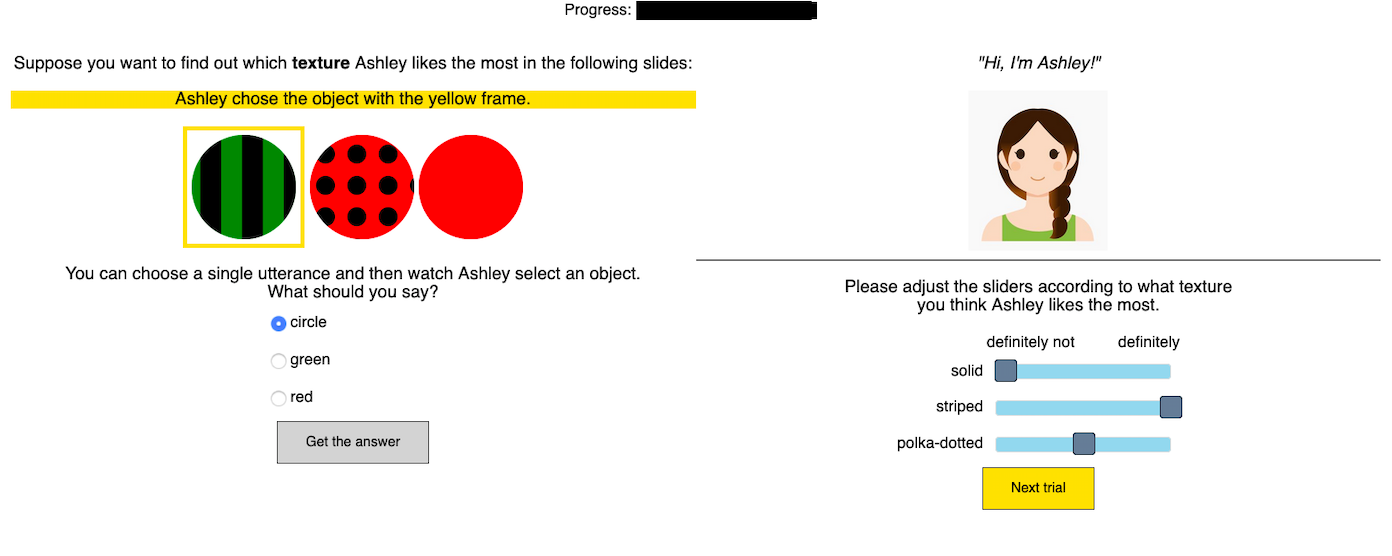
\includegraphics[width=5.5in]{images/trial.png}
	\caption{ \small{A sample trial. Each trial portrays a listener. The speaker (that is, the actual human participant) produces an utterance to refer to one of the objects. The simulated listener picks an object, which, as a result, is marked by a yellow outline. The participant then evaluates which preferences of the listener may have led her to the particular object choice, specifying the inference by adjusting the sliders for each of the features. Please note that we fully focus on the preference inference process in this paper, leaving the analysis of the utterance choice behavior for future work.} }
	\label{exp1-trial}
\end{figure*}



\subsection{Participants}

We recruited 100 participants with US IP addresses through Amazon.com's Mechanical Turk crowdsourcing service. Subjects were compensated for their participation. On the basis of a post-test demographics questionnaire, we identified 98 participants as native speakers of English. 3 participants reported that they did not understand the instructions or were confused by the task. As a result, the data from 95 participants was included in the analysis. We obtained a confirmation from all the subjects that they agree to participate in the study.


\subsection{Design and methods}

We presented the subjects with a series of reference game scenarios modeled after Figure~\ref{FG-ref-game} from \citeA{frankgoodman2012}. The experiment participant played the role of the speaker. Her task was to find out a certain type of preferences of the listener, either related to color of objects, their texture, or their shape. 
% Asya: I use the word 'texture' because that's what it says in Figure 2

Each trial consisted of 2 parts. 
First, the speaker had to select an utterance (left part of Figure~\ref{exp1-trial}) and watch the simulated listener pick an object. Listener's choices were driven by the literal semantics of the utterance, i.e. only red objects qualified as a possible choice following the utterance ``red'. We built in particular distributions of feature preferences giving a priority scale. The listener picked the object that matched the highest value on the scale. For example, when the scale was ``red $>$ green $>$ blue'', and all three colors were present in a scene and compatible with the utterance, the listener picked the red object. If only green and blue objects were present and qualified, the listener picked a green object. Listener names and which particular feature preferences the speaker needed to infer (color, shape or texture) were chosen randomly in each block but remained constant within a block.
Participants completed a series of 4 blocks, each containing 4 trials. 

In the second part of the trial (right half of Figure \ref{exp1-trial}), the speaker adjusted the sliders guessing the listener's preferences. Then the experiment proceeded to the next trial with the same simulated listener and the same hierarchy of preferences. The sliders remained in their adjusted positions, so the participant could see which preference inferences she had made so far.

Objects were allowed to vary along three dimensions: color (blue, red, green), shape (cloud, circle, square), and texture (solid, striped, polka-dotted). The list of utterances contained the properties of the three objects present, excluding the utterances that correspond to the target feature type (e.g. texture in Figure~\ref{exp1-trial}). All trials contained at least one ambiguous utterance option. 

%To compare the model predictions to the human data, we calculated an average value for each slider.
%, binning data into 48 ambiguity classes.
% for Experiment 1 and 14 classes for Experiment 2. 
%We excluded the sliders if their corresponding feature value was not present in a scene. For example, for the trial depicted in Figure \ref{exp1-trial}, we excluded the sliders for solid things and squares since none of these are present, and therefore no learning about them is possible.


%%% Martin: this is not necessary I believe since we do not do this anylonger: (?)
%We partitioned the data into ambiguity classes, similar to \citeA{frankgoodman2012}. Depending on how many features competitor objects share with the chosen object, we were able to identify 48 ambiguity classes, which group the constellations that have the exact same ambiguity pattern. The ambiguity classes distinguish how many objects are referenced by the utterance, how the referenced objects differ in their two non-uttered features, and how the non-referenced objects differ from the referenced objects and from each other. We excluded combinations that contained identical objects as well as combinations where objects share none of the features, i.e. all objects are unique, leaving us 33 classes in this experiment. Each ambiguity class yields unique model prediction values for the individual features present (with respect to their ``ambiguity role'' in the particular ambiguity class) in corresponding scenarios $S$, effectively distinguishing all model-relevant cases.

%For example, considering the top-left-most case, ,where the utterance ``red" refers to two possible objects and the choice falls onto one of them (here the red cloud), which shares one property with the other, not referenced object (its cloud shape), but no further properties with the other referenced object (neither its shape nor its pattern). Thus, its other property is unique (its striped pattern)
%If, as an alternative scenario, he utterance was ``green", only one object would qualify (the green, dotted cloud), preventing the learning about preferences. 
%In that case, the model would assign equal probability to the listener's preferring dotted objects, striped objects, clouds, and squares. 
%Once the model establishes that more than one object can be picked, it also needs to consider whether alternative objects share their features with the target object. For example, if both red objects were also striped, the model would not be able to infer any preferences about the pattern. 
%In addition to these considerations, ambiguity classes also distinguish whether the objects that are not referenced by the utterance share any of their feature values.



\section{Results}

In this experiment, the task of the participants was to first choose an utterance, then to observe the choice of an object, and ultimately to infer the hierarchy of the listener's preferences. Subjects performed these tasks in a series of four trials. We tested two main types of models with respect to the inferred preferences of the listener after observing her (simulated) object choice: an iterative Bayesian inference model takes into account the posterior estimates from the previous trial in one block as the next prior, and a non-iterative model, which assumes uniform preference priors for all trials.
Moreover, we compared the performance of these two models with a baseline model, which predicts uniform preference posteriors. 
We expected to see the largest difference between the two models in trial 4, where the performance difference between the iterative and the non-iterative model should be most-pronounced.


We optimized the two free parameters of the model--softness $\gamma$ and obedience $\beta$--at the global level, i.e. we obtained a single pair of estimates based on the data from all of the participants. 
Given the parameters, we calculate posterior preference model predictions and compare them with the human data. 

When comparing the model predictions for each trial with the human responses, correlation statistics can be determined. 
In Figure~\ref{iterative}, we plot the human data--slider values of individual trials--against the iterative model predictions. 
The iterative model captures a large proportion of variance in the human data  ($r^2=0.558$, $F(1,1138) = 1437$, $p<0.001$), while the non-iterative model (Figure \ref{non-iterative}) is less accurate at predicting the data  ($r^2=0.382$, $F(1,1138) = 703.5$, $p<0.001$).


\begin{figure}[t]
	\centering
	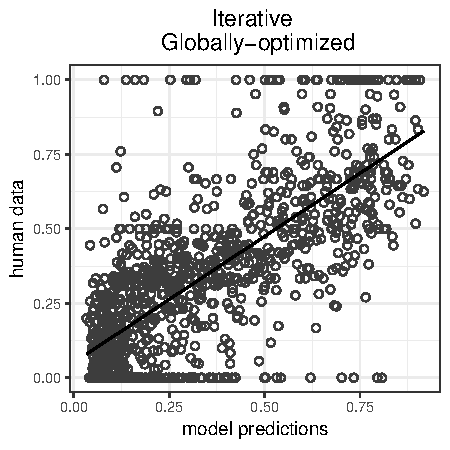
\includegraphics[width=.8\linewidth]{images/m4.pdf}
	\caption{Iterative model predictions with softness $\gamma$ and obedience $\beta$ optimized globally. Each data point represents a single trial.}	
	\label{iterative}
\end{figure}

 \begin{figure}[h]
	\centering
	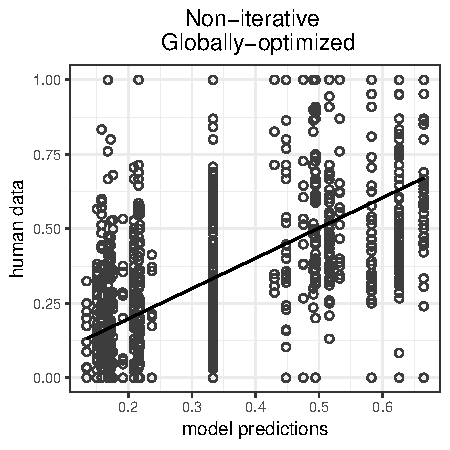
\includegraphics[width=.8\linewidth]{images/m8.pdf}
	\caption{Non-Iterative model predictions with softness $\gamma$ and obedience $\beta$ optimized globally. Each datapoint represents a single trial.}	
	\label{non-iterative}
\end{figure}
 
To further assess the performance of the two models we can examine the KL values that we obtained in the course of optimization.
For a point of comparison, we can use the KL for the uniform base model, which yields a value of $558.7$ when integrating all trials, where a large KL divergence term indicates a poor fit of a model since the KL divergence indicates the difference between the give participant data and the model predictions.
The iterative model produces a KL value of $318.4$ compared to $356.3$ for the non-iterative model. 
Since the KL divergence corresponds to the negative log-likelihood between the model and the data, we can interpret the difference between two KL values as a Bayes factor.
In our case we observe a Bayes factor of $37.9$ which corresponds to very strong evidence in favor of the iterative model on Jeffreys scale \cite{jeffreys1961theory,Lewandowsky:2011}.


We furthermore optimized the model's two parameters for each individual participant separately, which yields an even better KL value of $237.89$.
Although this difference may be considered not significant when compared to the globally optimized one due to the much larger number of free parameters (two per participant versus two in total), it is still interesting to consider the resulting correlation plot. 
Figure~\ref{iterative_individually} essentially confirms the fit of the globally-optimized version, yielding an event better correlation ($r^2=0.673$, $F(1,1138) = 2349$, $p<0.001$).
Thus, while the individually optimized mode appears to catch important individual differences, it adheres to the confirming trend that participants indeed pursue an iterative, approximately-Bayesian inference process. 



\begin{figure}[t]
	\centering
	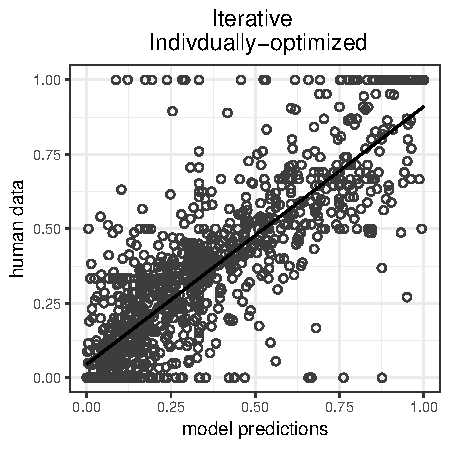
\includegraphics[width=.8\linewidth]{images/m2.pdf}
	\caption{Iterative model predictions with softness $\gamma$ and obedience $\beta$ optimized \emph{individually} for each participant. Each data point represents a single trial.}
		\label{iterative_individually}
\end{figure}

%In order to assess whether subjects learned the target ordering of listener preferences, we developed an evaluation score from 0 to 3. The preferences are encoded as pairs. If a hierarchy is $ a > b > c $, there are three relations to learn:  $ a > b$; $ b > c $, and $ a >  c $. A score of 3 is assigned if the relations in all the pairs are identified correctly, a score of 0 means that all the relations between feature preferences have been reversed, and values 1 and 2 correspond to 1 and 2 pairs guessed correctly respectively.
%
%Figure \ref{learning-success} reveals that both the model and the human subjects successfully learned the implemented hierarchy of preferences: both got the evaluation scores of 2 and 3 most of the time.
%
%\begin{figure}
%	\centering
%	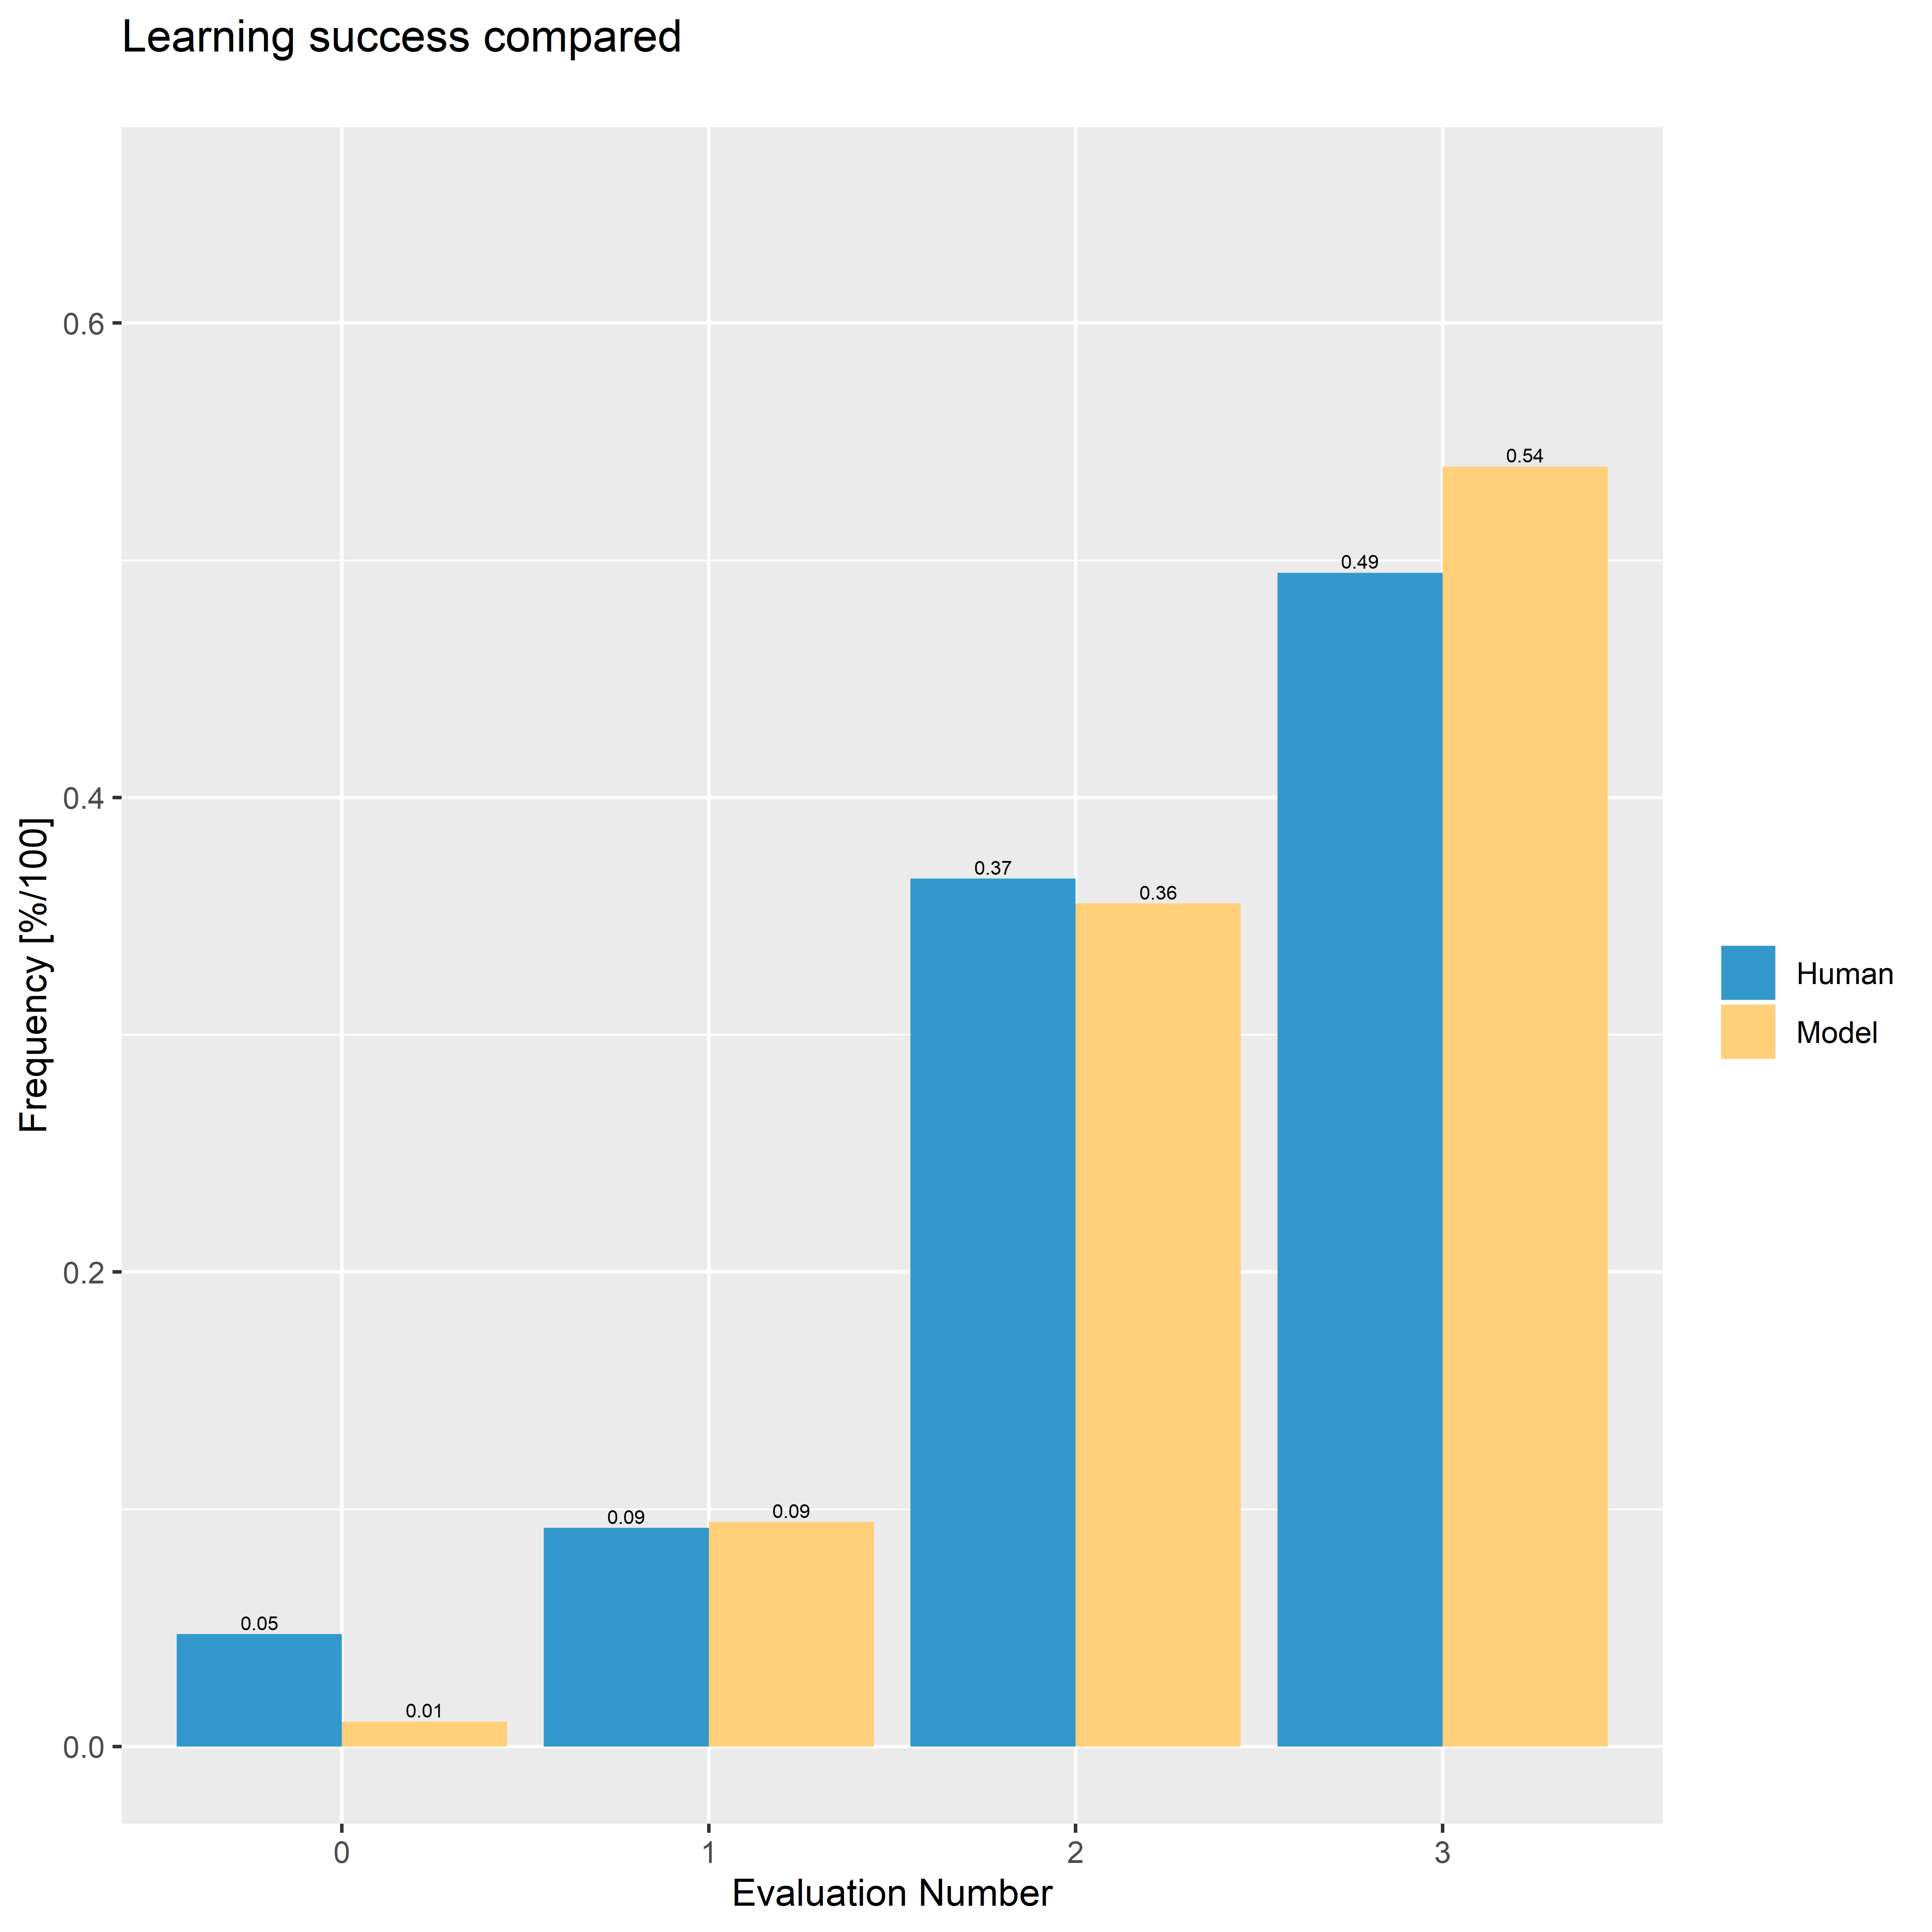
\includegraphics[width=.5\linewidth]{images/evalNumCompairPlotWithFirstBlock.png}
%	\caption{Success of human subjects and the model in detecting the listener preferences}
%	\label{learning-success}
%\end{figure}
%
%We can now explore how the accuracy of predictions improves over time. We predicted that if learning is iterative and subjects use the information about the preferences that they have already accumulated, we should see higher evaluation scores on subsequent trials. We see in Figure \ref{learning-progression} that the line for best evaluation score ``3'' rises as the trial order increases.
%
%\begin{figure}
%	\centering
%	\includegraphics[width=.5\linewidth]{images/LearningProcessLinePlot1.png}
%	\caption{Success of human subjects and the model in detecting the listener preferences}
%	% Martin: please leave in these details - this may appear slightly formal but very useful for the slightly more technical reader. 
%	\label{learning-progression}
%\end{figure}
%
%As both Figures \ref{learning-success} and \ref{learning-progression} show, in certain cases both the speakers and the model failed to learn the preferences hierarchy. We attribute this effect to different strategies participants used when choosing utterances. Recall, that while every trial contained at least one ambiguous utterance, participants also had a possibility to choose an unambiguous utterance. Unambiguous utterances pick a single object making the learning impossible both for human subjects and for the model (Figure \ref{learning-unambiguous}). When subjects pick ambiguous utterances, learning curve clearly goes up (Figure \ref{learning-ambiguous}).
%
%\begin{figure}
%	\centering
%	\includegraphics[width=.5\linewidth]{images/LearningProcessLinePlotHuman3.png}
%	\caption{Success of human subjects and the model in detecting the listener preferences}
%	% Martin: please leave in these details - this may appear slightly formal but very useful for the slightly more technical reader. 
%	\label{learning-unambiguous}
%\end{figure}
%
%\begin{figure}
%	\centering
%	\includegraphics[width=.5\linewidth]{images/LearningProcessLinePlotHuman2.png}
%	\caption{Success of human subjects and the model in detecting the listener preferences}
%	% Martin: please leave in these details - this may appear slightly formal but very useful for the slightly more technical reader. 
%	\label{learning-ambiguous}
%\end{figure}

\section{Discussion}

In order to interpret an ambiguous utterance, the listener needs to draw on her prior knowledge to decide which interpretation is most likely. This prior knowledge, broadly viewed, can include personal preferences and beliefs, as well as the understanding of the current context. Listener choices are in that sense informative about the underlying priors of the listener. 

We simulate the ambiguity resolution process with a Bayesian reasoning model that allows accumulation of evidence over a series of trials. The experimental data reveals that speakers are indeed able to infer hidden prior preferences by observing behavioral choices. Moreover, the model confirms that this process indeed unfolds in an accumulative manner, using the inferred posteriors as the next preference priors. 
Broadly speaking, this type of inference allows communicative partners to gain better understanding of each other, and to further anticipate how ambiguity maybe resolved.
The results are also in line with theories of social active inference \cite{Friston:2015b} but extend this rather general framework to the inference of motifs and preferences, besides the interesting fact that dialogues may be played-out in a co-confirming, duet-like manner. 


The presented computational model of the reasoning process takes into account iterative learning. It implements the idea that the accumulation of evidence may be realized by storing posteriors -- here, of preferences, but in general of any decision biases, including knowledge, which the listener may have -- and employing these stored posteriors as subsequent priors (here, over learned feature value preferences) to adjust them further in relevant, subsequent interactions. While we do observe a better performance of the iterative model compared to the model that assumes uniform priors for each trial, we also acknowledge the fact that there is still substantial variance in the data that the model was unable to capture when globally or individually optimizing for two free parameters. 
% Martin: there is no plot currently or data reported, which confirms the following statement :-(  :
% While the model successfully learns the relative hierarchy of preferences, 
A large part of this remaining difference may be explained by the fact that the model does not make any assumptions about the preference distribution of the listener. 
On the other hand, the human participants can deduce after the first trial that the simulated listener most likely has one most preferred feature value, one second most-preferred one, and one least preferred one. 
Thus, as long as the sliders are ordered accordingly, the answer can be considered correct from the participants' perspective, leaving lots of variance in the slider values. 
In fact, in order to model this ranked preference with PSIRSA, the preference estimates would need to be exponentially distributed on a rather extreme scale.
% , which is certainly not what the participants did, when they chose their slider values as indicators for ``preferences''. 
In future work, we thus intend to enhance PSIRSA to either explicitly model the expectation of ranked preference distributions or to modify the preference encoding to a logarithmic scale, which may correspond more closely to the slider value interpretation of our human participants. 

Nonetheless, we consider the gathered evidence as strongly hinting at iterative approximate Bayesian inference processes, which are at play when interpreting choices of dialogue participants. 
Although the current scenario is certainly rather abstract, we are convinced that interpretation choices unfold in natural dialogues all the time, relying on assumptions about the conversation partner's intentions, knowledge, and preferences as well as the actual own ones. 
We thus hope to extend the proposed framework to even more natural settings in the near future, where true dialogues about a particular topic -- such as a short story -- unfold and conversation partners draw conclusions not only about untold parts of the story but also about the knowledge of their conversation partner when interpreting and generating respective sentences.






 %We demonstrate that if ambiguous utterances are chosen, the accuracy of guesses improves as a function of trial order, and we faithfully model this process computationally. 


%\section*{Funding}
%
%This project has been funded by the Deutsche Forschungsgemeinschaft (DFG, German Research Foundation)--Project number 198647426. 
%
%\section*{Data availability}
%Data supporting the findings of this study are available from the corresponding author upon request.

\bibliographystyle{apacite}
\setlength{\bibleftmargin}{.125in}
\setlength{\bibindent}{-\bibleftmargin}

\bibliography{prior-inference}


\end{document}

